% Template für Checkboxen ----
\newcommand{\checkbox}[1]{
\ifx#1\undefined
  $\Box$
\else
  $\boxtimes$  
\fi}
%----------------------------

\maketitle

% -------------------------------
% WAS
% -------------------------------
\section*{Was}

\subsection*{Problem}
\desc

\subsection*{Lösung}
\solution

\subsection*{Grafische Darstellung}
\begin{figure}[H]
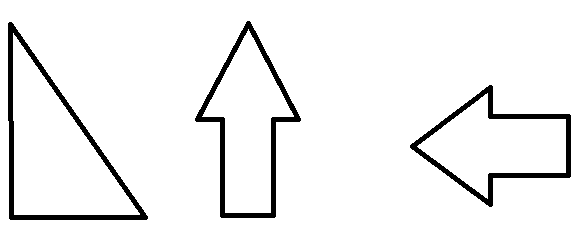
\includegraphics[scale=0.3]{mypicture.png}
\end{figure}

\subsection*{Kategorie}
\ifthenelse{\equal{\category}{give}}{$\boxtimes$}{$\Box$} Give \\
\ifthenelse{\equal{\category}{take}}{$\boxtimes$}{$\Box$} Take \\
\ifthenelse{\equal{\category}{exchange}}{$\boxtimes$}{$\Box$} Exchange \\
\ifthenelse{\equal{\category}{extend}}{$\boxtimes$}{$\Box$} Extend \\
\ifthenelse{\equal{\category}{connect}}{$\boxtimes$}{$\Box$} Connect


% -------------------------------
% WIE
% -------------------------------

\section*{Wie}

\subsection*{Aktion des Benutzers}
\useraction

\subsection*{Reaktion des Sende-und Empfänger-Gerätes}
\reaction

\subsubsection*{Reaktion im Erfolgsfall:}
\checkbox{\reactionSuccessVisual} visuelle Rückmeldung \\
\checkbox{\reactionSuccessAcustic} akustische Rückmeldung, z.B. Ton \\
\checkbox{\reactionSuccessSensitive} sensitive Rückmeldung, z.B. Vibration \\

\subsubsection*{Reaktion im Nicht-Erfolgsfall:}
\checkbox{\reactionFailureConnection} wenn keine funktionierende Verbindung besteht \\
\checkbox{\reactionFailureNoDevice} wenn das Zielgerät nicht erkannt wurde \\
\checkbox{\reactionFailureCompatibility} wenn das Zielgerät nicht kompatibel ist

\subsection*{Hinweise zur Gestaltung der Interaktion}
\designnotes

% -------------------------------
% WANN
% -------------------------------

\section*{Wann}

\subsection*{Geeigneter Nutzungskontext}

\subsubsection*{Zeit}

\checkbox{\simultaneously} gleichzeitige Nutzung von Geräten \\
\checkbox{\sequentially} sequentielle Nutzung von Geräten 

\subsubsection*{Modus}
\checkbox{\online} online \\
\checkbox{\offline} offline 

\subsubsection*{Ort}
\checkbox{\private} privat \\
\checkbox{\semipublic} halb-öffentlich \\
\checkbox{\public} öffentlich \\
\checkbox{\stationary} stationär \\
\checkbox{\onthego} unterwegs 

\subsubsection*{Position}
\checkbox{\leanback} Lean-Back \\
\checkbox{\leanforward} Lean-Forward 


\subsubsection*{Teilnehmer}
\checkbox{\single} Einzelnutzer \\
\checkbox{\collaboration} Kollaboration 

\subsubsection*{Tätigkeit}
\checkbox{\smalltask} kleinere Aufgabe \\
\checkbox{\repeatedtask} wiederholte Tätigkeit \\
\checkbox{\locationbased} ortsbezogene Informationsbeschaffung \\
\checkbox{\distraction} Ablenkung \\
\checkbox{\urgent} dringendes 

\validcontext

\subsection*{Abzuratender Nutzungskontext}
\notvalidcontext

\subsection*{Geräteklassen}
\devicetabular

\subsection*{Entfernung zwischen Sender- und Empfänger-Gerät}
\checkbox{\distanceA} Entfernung 1 \\
\checkbox{\distanceB} Entfernung 2 \\
\checkbox{\distanceC} Entfernung 3 \\
\checkbox{\distanceD} Entfernung 4 

% -------------------------------
% WARUM
% -------------------------------

\section*{Warum}

\checkbox{\established} Bewährtes Interaction Pattern \\
\checkbox{\candidate} Interaction Pattern Kandidat 
\checkbox{\realizable} realisierbar
\checkbox{\futuristic} futuristisch 

\subsection*{Analoge Patterns}
\otherpatterns

\subsection*{State of the Art/Gebrauchshistorie}
\stateoftheart

\subsection*{Checkliste: Entspricht die Interaktion der Definiton eines "Blended Interaction"?}
\checkbox{\designprinciples} Werden die Designprinzipien berücksichtigt?
\begin{itemize}
\item[-] Die Interaktion findet in Kombination mit physikalischen Gegenständen statt.
\item[-] Die Interaktion kann in einer Kollaboration ausgeführt werden.
\item[-] Die Interaktion unterstützt einen Workflow/eine Aufgabe.
\item[-] Die Interaktion findet in einer physikalischen Umgebung statt.
\end{itemize}

\checkbox{\imageschemata} Image Schema/ta liegen zu Grunde.
\begin{itemize}
\item[-] \checkbox{\imageschemataA} Image Schema 1
\item[-] \checkbox{\imageschemataB} Image Schema 2
\item[-] \checkbox{\imageschemataC} Image Schema 3
\end{itemize}

\checkbox{\realworld} Die real-weltlichen Kenntnisse des Menschen werden berücksichtigt.
\begin{itemize}
\item[-] \checkbox{\realworldA} Naive Physik
\item[-] \checkbox{\realworldB} Body Awareness and Skills
\item[-] \checkbox{\realworldC} Environment Awareness and Skills
\item[-] \checkbox{\realworldD} Social Awareness and Skills
\end{itemize}

\checkbox{\metaphor} Es ist eine natürliche Interaktion. Metapher/Assoziation: 

% -------------------------------
% TECHNISCHES
% -------------------------------

\section*{Technisches}

\subsection*{Technologien zur Objekterkennung}
\checkbox{\technologyObjectA} Distanz A \\
\checkbox{\technologyObjectB} Distanz B \\
\checkbox{\technologyObjectC} Distanz C \\
\checkbox{\technologyObjectD} Distanz D \\

\technologyObjectDesc

\subsection*{Technologien zur Kommunikation}
\checkbox{\technologyCommunicationServer} Server-basiert \\
\checkbox{\technologyCommunicationAdhoc} Ad-hoc-Netzwerk basiert\\

\technologyCommunicationDesc

\subsection*{Technologien zur Bewegungs-/Orientierungsbestimmung}
\checkbox{\technologyOrientationAccelerometer} Accelerometer \\
\checkbox{\technologyOrientationGPS} GPS \\
\checkbox{\technologyOrientationGyroskop} Gyroskop \\
\checkbox{\technologyOrientationAnnaeherung} Annäherungssensor \\
\checkbox{\technologyOrientationHoehe} Höhenmesser \\
\checkbox{\technologyOrientationBeacons} Beacons \\
\checkbox{\technologyOrientationOther} andere: \\

\technologyOrientationDesc{...} 

\subsection*{Prototyp/Lösungsansatz/Code-Snippets/UML-Diagramm}
\prototype



% -------------------------------
% SONSTIGES
% -------------------------------

\section*{Sonstiges}

\subsection*{Autor/en}
\authors

\subsection*{Literaturreferenzen}
\literature

\subsection*{Abbildungsverzeichnis}
\figures

\subsection*{Versionshistorie}
\versionhistory

\subsection*{Kommentare}
\comments

\subsection*{Offene Fragen}
\questions